\chapter{Plugin system}
\vspace{-10mm}

There was a need of image segmentation support in Dicom-Presenter. A few of FNSPE student are working on image segmentation algorithms of MRI images. Therefore, an idea to import these algorithms into Dicom-Presenter has risen. The best idea was to design a plugin system for importing segmentation algorithms.
Plugin in computer sciences is an optional addition to some application. It is not usually distributed with application itself, but can be added by user according to their needs. An example of a plugin can be an additional python script to Gimp program which allows user to apply 'sepia effect' on his photos. According to the mentioned example, plugins can be written in another language than application itself, they obtain some new functionality to application.


All segmentation algorithms developed at FNSPE were written in C language due to its performance. Plugins in C language are compiled to a Dynamic-Link libraries and run-time loaded. A theory of C++ libraries and description of run-time loading libraries can be found in Section \ref{library}.

\section{Image Segmentation Algorithms}

\red{
Popsat algoritmy Kuby Louckeho a Radka Maci.\\
}

\section{Plugins System Requirements}

It is needed to set rules for plugin libraries. Thereafter, a library following these rules should be applicable in Dicom-Presenter. The first thing is to generalize what the libraries will need as an input and output. All three libraries made by FNSPE students required an image with designated segmentable area together with computational parameters as an input. The most reasonable way to insert computation parameters is to generate a GUI interface including required input elements. This chapter discusses plugins GUI construction done at the application runtime and its connection to the loaded plugin library. A plugin interface was considered to be as simple as possible - a key idea was to require a minimum of source code modifications in existing image segmentation libraries.

\section{Generating Plugins GUI}

Dicom-Presenter's graphic user interface is built with use of Qt framework. Objects of Qt library classes represent application control elements. The objects can be created and displayed at a runtime according to plugin needs. A mandatory question is which way to choose for plugin GUI description.

Qt library offers its own format of GUI description. There is a tool in Qt SDK\footnote{Qt Software Development Kit is a package for Qt based applications development. SDK includes library files together with a native development IDE.}, which offers an interactive GUI creation. It produces a XML file which describes the GUI. A strong argument for using this solution is that Qt library offers native tools for processing generated GUI description files.

Another possible way is to declare own language for GUI description. Firstly, it was implemented easily: Lines in a description file were corresponding to GUI elements. First word of a line determined a type of an element. Other words on the line described element's properties such as default value, minimum and maximum value or matching function in a library. The second step was a transformation to XML standards. The result was similar to preceding option but distinctive in syntax and naming. 

It would seem that the first solution is more reasonable. No new language is declared, though existing Qt library standard is used. Unfortunately, the Qt library syntax was primarily supposed to be generated by automated tool. The XML code is too complicated to be written manually - there are too much required phrases in the code. Moreover, GUI elements are described by class-names from Qt library - therefore, it is needed to know the Qt library to be able to write a description manually. The only option would be to generate GUI description by the Qt interactive tool. However, it is a complex tool, aimed for creating extensive GUI layouts for large applications. Unlike, segmentation algorithm plugins require only a few control elements (input fields and buttons). It seems more accessible for a programmer to follow a few rules declared in GUI description language created for Dicom-Presenter instead of following extensive number of rules attached to Qt GUI description language.

\subsection{Dicom-Presenter GUI Description Language}

The GUI description should determine types of control elements and their layout in interface window. The language for Dicom-Presenter GUI description is supposed to be simple. For every numeric input field it is needed to know: a required variable type (integer or float), the minimal and maximal possible value, the default value, a parameter description. Passing char parameters was realized by a combobox element - all possible values are listed in a dropdown menu.

A numeric field is declared by a string:

\clist{<numinput type="..." min="..." max="..." default="..." name="..."/>}

Where \clist{type} determines a C/C++ type (integer of double), \clist{min}, \clist{max}, \clist{default} determine minimum, maximum and default value and \clist{name} determines a parameter description.

A combobox can be declared in a similar way like in (X)HTML:

\noindent \indent \clist{<combobox type="..." name="...">}\\
\indent \indent \clist{<option value="..." name="..."/>}\\
\indent \indent \clist{<option value="..." name="..."/>}\\
\indent \clist{</combobox>}

Where \clist{type} determines a variable type passed to a library. \clist{name} in \clist{combobox} tag is a text description of property. The \clist{name} property in \clist{option} tag is a text description of a \clist{value} which is passed to a library.

An example GUI description file can be seen in Table \ref{tab:exampledescription}. The process of parsing a description file is illustrated on Listing \ref{parsingdescription} - the code refers to parsing information about a numeric input. Notable is the use of \clist{dymanic\_cast} operator, which allows unification of two different pointers, if the classes inherit the same parent.

\lstset{numbers=none,frame=none}

\begin{table}[ht]
	\caption{An example of a Dicom-Presenter plugin's GUI and its description.\label{tab:exampledescription}}
	\begin{tabular}{|m{\textwidth}|}
	\hline
\begin{lstlisting}[language=xml,morekeywords={zzz,ADD_EXECUTABLE,add_custom_command,add_library,target_link_libraries,OUTPUT,COMMAND,xxx})]
<xml>
  <numinput type="int" min="0" max="10" name="Lambda" function="lmbd"/>
  <numinput type="int" min="0" max="20" name="Sigma" function="sgm"/>
  <combobox type="char" name="Algorithm" function="algorithm">
    <option value="a" name="Modified algorithm"/>
    <option value="p" name="Original algorithm"/>
  </combobox>
  <button function="main" name="Run"/>
</xml>
\end{lstlisting}
		\\
		  \hline		
		  \noalign{\smallskip}
			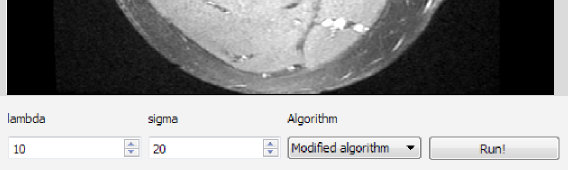
\includegraphics[width=\textwidth]{Text/IMG/Plugins.png}
		\\
		\hline
		\end{tabular}
\end{table}%

\lstset{numbers=left,frame=single,}

\begin{lstlisting}[caption={Parsing data from a description file - integer input.}, language=C++,label=parsingdescription,morekeywords={zzz,ADD_EXECUTABLE,add_custom_command,add_library,target_link_libraries,OUTPUT,COMMAND,xxx})]
if (type=="int"||type=="double"){
	if (tag=="numinput") {
		QSpinBox *spinbox = new QSpinBox();
		...
		ControlerTable[i]=dynamic_cast<QWidget*>(spinbox); 
		Layout->addWidget(spinbox,1,y);
	}	
	if (tag=="combobox"){
		QComboBox *combobox = new QComboBox();
		if (e.hasChildNodes()){
			QDomNodeList childs=e.childNodes();
			for (int k=0; k<childs.count(); k++){
				QDomNode n = childs.at(k);
				QDomElement el = n.toElement();
				combobox->addItem(element.attribute("name"),element.attribute("value"));
			}					
		}
		ControlerTable[i]=dynamic_cast<QWidget*>(combobox); 
		Layout->addWidget(combobox,1,y);
		...
	}
	...	
}
\end{lstlisting}




%\subsection{Implementation of user interaction}



\section{Dynamically Loading Plugin Functions}

Dicom-Presenter's image segmentation algorithms use individual parameters. Therefore, each main computational function in each plugin needs individual number and types of parameters. A C/C++ function located in dynamically loaded library is ran through a function pointer as seen on Listing \ref{sec:runtimeloading}. This pointer must have a fixed number and fixed types of parameters given at compilation. Thus, it is not possible to call various functions with various sets of parameters from a dynamically loaded library. It is possible to run only a finite number of types of functions according to a set of given parameters. There were several solutions how to make the Dicom-Presenter's plugin system variable enough to load and run previously unknown functions:

\begin{enumerate}
\item It is possible to pre-define sufficient number of function pointer types at a compilation time. Then, each Dicom-Presenter plugin must have input function of predefined type.
\item Another solution is based on a fact that a function pointer can have more parameters than targeted function. For example, a function pointer having five integer parameters can point to a function receiving only three integer parameters - the last two given parameters will be ignored. Therefore it would be possible to define function pointers with excessing number of float, integer and char parameters. A function pointer would be assigned to a function to fit the first couple of parameters and ignoring the rest.
\item Another applicable way is to allow only one-parameter requiring functions to be present in a plugin. If the algorithm would need more parameters, then appropriate functions settings these parameters would be ran. Parameters can be saved as global variables to be reachable by main computational function. This solution has a great advantage: It is possible to call the parameter setting functions simultaneously to user manipulating with relevant GUI elements. Then, an instant feedback from the library could be present (checking for incompatible values). This solution was implemented but it seemed too restrictive for library design. 
\item Next option is inspired by passing command line arguments to a standard C/C++ application. C/C++ Main Function receives a pointer to an array of all arguments. As in this case a plugin library function can receive three pointers to three array types: pointer to int, pointer to double and pointer to char. The arrays can be of any length.
\item Last option is to pass all parameters in a string. This option requires the plugin library to parse strings of some given format. 
\end{enumerate}

At first the third option was used in implementation. Function setting algorithm parameters were called while setting parameters in GUI. But there were no real benefits of library response while setting GUI parameters. More than that, the rules for plugins were too bounding. 

Another reasonable option was nr. 5 - passing parameters in a string. The advantage is a flexibility of the system. On the other hand, image segmentation libraries will predominantly require numeric parameters. So, two conversions between numbers and strings would be needed.

Therefore, the final version of plugin API was implemented using option 4. The main function of a library receives pointers to three arrays where all parameters are saved. An illustration of the source code of this solution is on Listing \ref{parameters}.

\begin{lstlisting}[caption={A process of passing parameters to the main computational function of a library.}, language=C++,label=parameters,morekeywords={zzz,ADD_EXECUTABLE,add_custom_command,add_library,target_link_libraries,OUTPUT,COMMAND,xxx})]
typedef bool mainFunction(int*,char*,double*);
int *argi;
char *argc;
double *argd;
...
argi[0]=10;
argi[1]=20;
....
ProcessAdress = GetProcAddress("main");
mainFunction* func=(mainFunction*)ProcessAdress;
func(argi,argc,argd);
\end{lstlisting}

\section{User interaction in Image Segmentation plugins}
As mentioned before, FNSPE image segmentation algorithms require computational parameters and an input image with designated area to be segmented. The segmentable area is defined by an initial curve. The entire initial curve has to be placed inside the segmentable area. The curve is then used as a set of initial values for algorithm. Mostly, the curve is iteratively expanded until it traces the area border. Then, the expanded curve fully defines the segmented area.

The initial curve had to be defined by the user somehow. The most user-friendly way would be to allow the user to paint the initial curve right inside the segmented image using a pointing device (computer mouse, touchscreen, etc.) Qt library offers extensive possibilities to perform free-hand painting into an image.

\subsection{Implementation of User Interaction}

Any mouse-control task in a computer application is mostly implemented according to the following schema: mouse movements are tracked by the application and redirected to a proper class, the actual mouse pointer position is obtained, an action based on the actual movement is performed and mouse movements are tracked again. The process is illustrated on Listing \ref{mousetrack}.

\begin{lstlisting}[label=mousetrack,caption={xxxx},escapeinside={@}{@}]
iDrawLabel = new drawLabel();
iDrawLabel->setMouseTracking(true);
...
void drawLabel::mousePressEvent(QMouseEvent* event){
	if (event->button()==Qt::LeftButton) pressedButton = leftButton;
	if (event->button()==Qt::RightButton) pressedButton = rightButton;
}
void drawLabel::mouseMoveEvent(QMouseEvent* event){
	if (pressedButton==noButton) return;
	int x = event->x();
	int y = event->y();
	if (pressedButton==leftButton){
		QPainter painter((QPaintDevice*)pixmap());
		painter.setPen(QPen(Qt::white, 5, Qt::SolidLine, Qt::RoundCap,Qt::RoundJoin));
		painter.drawEllipse (x,y,5,5);
	}
	update();
}
void drawLabel::mouseReleaseEvent(QMouseEvent* event){
	pressedButton = noButton;
}
\end{lstlisting}

There are three functions related to mouse actions in the example \ref{mousetrack}: \clist{mousePressEvent}, \clist{mouseMoveEvent}, \clist{mouseReleaseEvent}. All the three functions are originally defined in Qt library and can be overloaded the demonstrated way. Qt framework ensures event-based calling of these overloaded functions. \clist{mousePressEvent} and \clist{mouseReleaseEvent} functions are called to avoid performing in \clist{mouseMoveEvent} action if no mouse-button is pressed. In fact, the \clist{QMouseEvent} object includes information about pressed buttons, therefore \clist{mousePressEvent} and \clist{mouseReleaseEvent} function calls could be eliminated. But it is a unique feature of Qt library; therefore, this implementation is more frequent.

\red{Pridat kod o generovani uzivatelskeho rozhrani}
\red{Pridat kod o predavani parametru funkcim}